% ---- p2-namespaced TikZ styles (package loading happens in preamble.txt) ----
\tikzset{
  p2ent/.style={circle, draw=black!65, line width=0.7pt, minimum size=9.5mm,
                inner sep=0pt, font=\small\bfseries},
  p2lab/.style={font=\scriptsize},
  p2rel/.style={draw=black!65, line width=0.7pt},
  p2el/.style={font=\scriptsize, fill=white, inner sep=1.5pt},
}
\newcommand{\pTwoTgt}{orange!22}
\newcommand{\pTwoAgt}{blue!12}
\newcommand{\pTwoAtt}{green!14}
\newcommand{\pTwoVen}{purple!12}

\subsection*{3. Network schemas and meta-paths}
\label{p2:sec:schemas}

Each schema below is $T_G=(\mathcal{A},\mathcal{R})$ for one benchmark family: circles are node
types (letter = the initial used in meta-path notation), edges are relation types. Inverse
relations are omitted for readability.

\begin{figure}[htbp]
\centering
\begin{minipage}{0.48\textwidth}\centering
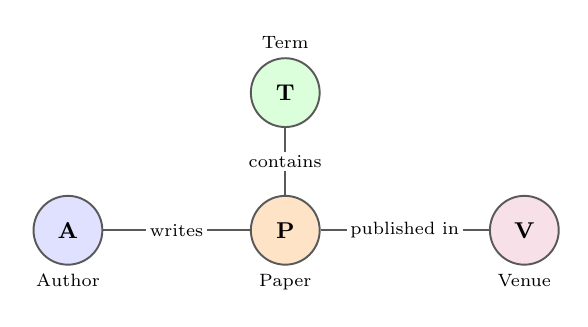
\begin{tikzpicture}[scale=0.92, every node/.style={transform shape}]
  \node[p2ent, fill=\pTwoTgt, label={[p2lab]below:Paper}]  (P) at (0,0) {P};
  \node[p2ent, fill=\pTwoAgt, label={[p2lab]below:Author}] (A) at (-3.0,0) {A};
  \node[p2ent, fill=\pTwoVen, label={[p2lab]below:Venue}]  (V) at (3.3,0) {V};
  \node[p2ent, fill=\pTwoAtt, label={[p2lab]above:Term}]   (T) at (0,1.9) {T};
  \draw[p2rel] (A) -- node[p2el]{writes} (P);
  \draw[p2rel] (P) -- node[p2el]{published in} (V);
  \draw[p2rel] (P) -- node[p2el]{contains} (T);
\end{tikzpicture}
\\[2pt]{\small\textbf{DBLP}}
\end{minipage}\hfill
\begin{minipage}{0.48\textwidth}\centering
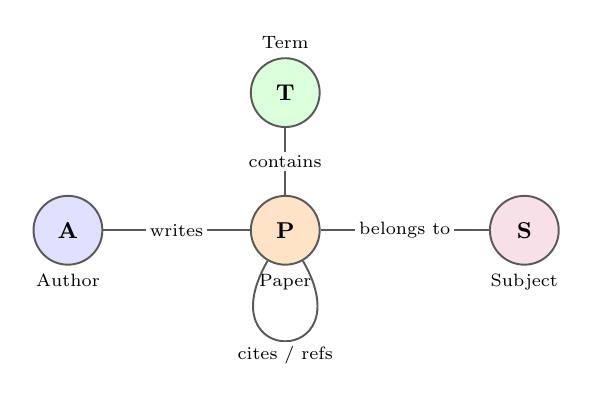
\begin{tikzpicture}[scale=0.92, every node/.style={transform shape}]
  \node[p2ent, fill=\pTwoTgt, label={[p2lab]below:Paper}]   (P) at (0,0) {P};
  \node[p2ent, fill=\pTwoAgt, label={[p2lab]below:Author}]  (A) at (-3.0,0) {A};
  \node[p2ent, fill=\pTwoVen, label={[p2lab]below:Subject}] (S) at (3.3,0) {S};
  \node[p2ent, fill=\pTwoAtt, label={[p2lab]above:Term}]    (T) at (0,1.9) {T};
  \draw[p2rel] (A) -- node[p2el]{writes} (P);
  \draw[p2rel] (P) -- node[p2el]{belongs to} (S);
  \draw[p2rel] (P) -- node[p2el]{contains} (T);
  \draw[p2rel] (P) to[out=-60,in=-120,looseness=9] node[p2el,below]{cites / refs} (P);
\end{tikzpicture}
\\[2pt]{\small\textbf{ACM}}
\end{minipage}

\vspace{10pt}
\begin{minipage}{0.48\textwidth}\centering
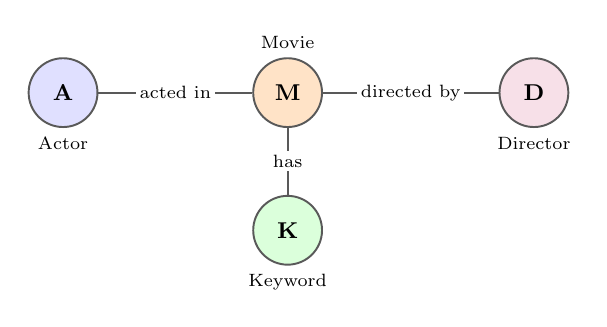
\begin{tikzpicture}[scale=0.92, every node/.style={transform shape}]
  \node[p2ent, fill=\pTwoTgt, label={[p2lab]above:Movie}]    (M) at (0,0) {M};
  \node[p2ent, fill=\pTwoAgt, label={[p2lab]below:Actor}]    (A) at (-3.1,0) {A};
  \node[p2ent, fill=\pTwoVen, label={[p2lab]below:Director}] (D) at (3.4,0) {D};
  \node[p2ent, fill=\pTwoAtt, label={[p2lab]below:Keyword}]  (K) at (0,-1.9) {K};
  \draw[p2rel] (M) -- node[p2el]{acted in} (A);
  \draw[p2rel] (M) -- node[p2el]{directed by} (D);
  \draw[p2rel] (M) -- node[p2el]{has} (K);
\end{tikzpicture}
\\[2pt]{\small\textbf{IMDB}}
\end{minipage}\hfill
\begin{minipage}{0.48\textwidth}\centering
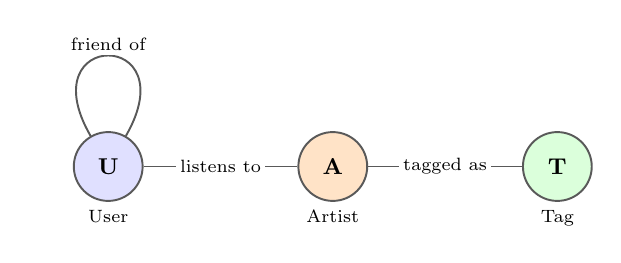
\begin{tikzpicture}[scale=0.92, every node/.style={transform shape}]
  \node[p2ent, fill=\pTwoAgt, label={[p2lab]below:User}]   (U) at (-3.1,0) {U};
  \node[p2ent, fill=\pTwoTgt, label={[p2lab]below:Artist}] (A) at (0,0) {A};
  \node[p2ent, fill=\pTwoAtt, label={[p2lab]below:Tag}]    (T) at (3.1,0) {T};
  \draw[p2rel] (U) -- node[p2el]{listens to} (A);
  \draw[p2rel] (A) -- node[p2el]{tagged as} (T);
  \draw[p2rel] (U) to[out=120,in=60,looseness=9] node[p2el,above]{friend of} (U);
\end{tikzpicture}
\\[2pt]{\small\textbf{LastFM}}
\end{minipage}

\vspace{10pt}
\begin{minipage}{0.54\textwidth}\centering
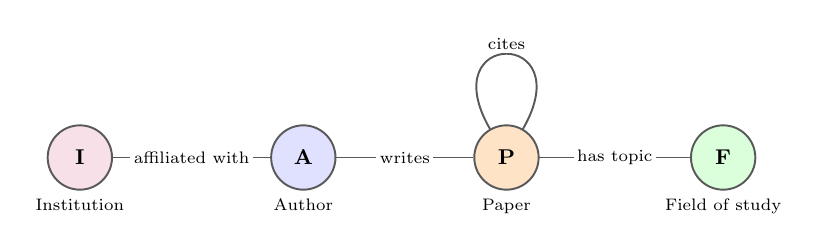
\begin{tikzpicture}[scale=0.86, every node/.style={transform shape}]
  \node[p2ent, fill=\pTwoVen, label={[p2lab]below:Institution}]    (I) at (-6.3,0) {I};
  \node[p2ent, fill=\pTwoAgt, label={[p2lab]below:Author}]         (A) at (-3.0,0) {A};
  \node[p2ent, fill=\pTwoTgt, label={[p2lab]below:Paper}]          (P) at (0,0) {P};
  \node[p2ent, fill=\pTwoAtt, label={[p2lab]below:{Field of study}}] (F) at (3.2,0) {F};
  \draw[p2rel] (A) -- node[p2el]{affiliated with} (I);
  \draw[p2rel] (A) -- node[p2el]{writes} (P);
  \draw[p2rel] (P) -- node[p2el]{has topic} (F);
  \draw[p2rel] (P) to[out=120,in=60,looseness=9] node[p2el,above]{cites} (P);
\end{tikzpicture}
\\[2pt]{\small\textbf{\texttt{ogbn-mag} / MAG240M}}
\end{minipage}\hfill
\begin{minipage}{0.44\textwidth}\centering
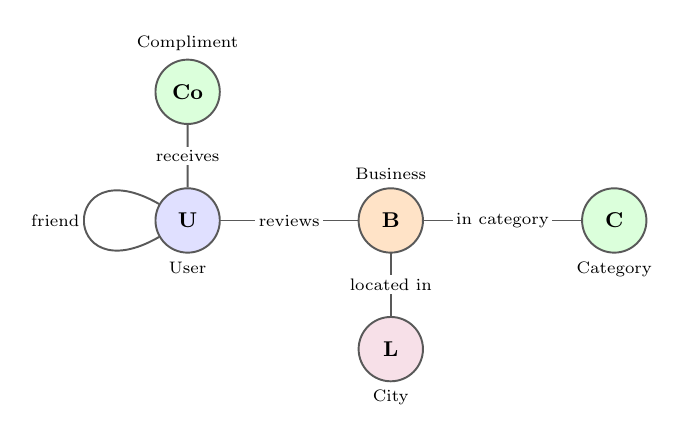
\begin{tikzpicture}[scale=0.86, every node/.style={transform shape}]
  \node[p2ent, fill=\pTwoTgt, label={[p2lab]above:Business}] (B) at (0,0) {B};
  \node[p2ent, fill=\pTwoAgt, label={[p2lab]below:User}]     (U) at (-3.0,0) {U};
  \node[p2ent, fill=\pTwoAtt, label={[p2lab]below:Category}] (C) at (3.3,0) {C};
  \node[p2ent, fill=\pTwoVen, label={[p2lab]below:City}]     (L) at (0,-1.9) {L};
  \node[p2ent, fill=\pTwoAtt, label={[p2lab]above:Compliment}] (O) at (-3.0,1.9) {Co};
  \draw[p2rel] (U) -- node[p2el]{reviews} (B);
  \draw[p2rel] (B) -- node[p2el]{in category} (C);
  \draw[p2rel] (B) -- node[p2el]{located in} (L);
  \draw[p2rel] (U) -- node[p2el]{receives} (O);
  \draw[p2rel] (U) to[out=150,in=210,looseness=9] node[p2el,left]{friend} (U);
\end{tikzpicture}
\\[2pt]{\small\textbf{Yelp}}
\end{minipage}

\vspace{10pt}
\begin{minipage}{0.7\textwidth}\centering
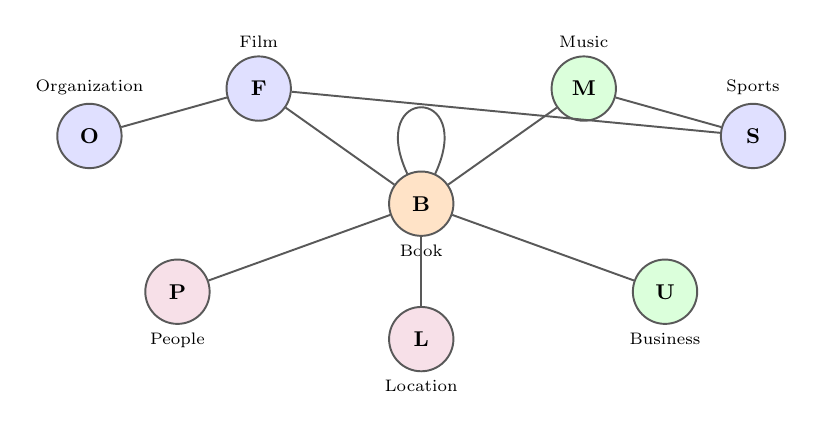
\begin{tikzpicture}[scale=0.86, every node/.style={transform shape}]
  \node[p2ent, fill=\pTwoTgt, label={[p2lab]below:Book}]         (B) at (0,0) {B};
  \node[p2ent, fill=\pTwoAgt, label={[p2lab]above:Film}]         (F) at (-2.4,1.7) {F};
  \node[p2ent, fill=\pTwoAtt, label={[p2lab]above:Music}]        (M) at (2.4,1.7) {M};
  \node[p2ent, fill=\pTwoVen, label={[p2lab]below:People}]       (Pe) at (-3.6,-1.3) {P};
  \node[p2ent, fill=\pTwoVen, label={[p2lab]below:Location}]     (L) at (0,-2.0) {L};
  \node[p2ent, fill=\pTwoAtt, label={[p2lab]below:Business}]     (Bu) at (3.6,-1.3) {U};
  \node[p2ent, fill=\pTwoAgt, label={[p2lab]above:Sports}]       (S) at (4.9,1.0) {S};
  \node[p2ent, fill=\pTwoAgt, label={[p2lab]above:Organization}] (O) at (-4.9,1.0) {O};
  \draw[p2rel] (B) -- (F);  \draw[p2rel] (B) -- (M);
  \draw[p2rel] (B) -- (Pe); \draw[p2rel] (B) -- (L);
  \draw[p2rel] (B) -- (Bu); \draw[p2rel] (F) -- (O);
  \draw[p2rel] (F) -- (S);  \draw[p2rel] (M) -- (S);
  \draw[p2rel] (B) to[out=115,in=65,looseness=9] (B);
\end{tikzpicture}
\\[2pt]{\small\textbf{Freebase (HGB)} --- 8 types, 36 relations; a representative subset is drawn.}
\end{minipage}
\caption{}
\label{p2:fig:schemas}
\end{figure}

\begin{table}[htbp]
\centering
\small
\caption{}
\label{p2:tab:metapaths}
\begin{tabular}{llp{7.6cm}}
\toprule
Dataset & Meta-paths & Semantics \\
\midrule
DBLP & APA & two authors co-wrote a paper (co-authorship) \\
     & APCPA / APVPA & two authors published at the same venue (community) \\
     & APTPA & two authors used the same term (topical similarity) \\
\midrule
ACM  & PAP & two papers share an author \\
     & PSP & two papers share a subject \\
     & PcPAP, PrPSP & HGB variants routed through a citation (c) or reference (r) hop \\
\midrule
IMDB & MAM & two movies share an actor \\
     & MDM & two movies share a director \\
     & AMA, DMD & two actors co-starred / two directors share a movie \\
\midrule
\texttt{ogbn-mag} & PAP & two papers share an author \\
     & PAIAP & two papers from the same institution (via author--institution) \\
\midrule
LastFM & UAU & two users listen to the same artist \\
     & UATAU & two users like artists sharing a tag \\
     & AUA, ATA & two artists share a listener / a tag \\
\midrule
Yelp & UBU & two users reviewed the same business \\
     & UBCaBU & two users reviewed businesses of the same category \\
\midrule
Freebase & BB, BFB, BPB & book--book; books sharing a film / a person \\
\bottomrule
\end{tabular}
\end{table}

\clearpage
% =====================================================================
